\documentclass[12pt,onecolumn]{article}
\usepackage[utf8]{inputenc} % UTF8 input encoding
\usepackage[T2A]{fontenc}   % T2A font encoding for Cyrillic script
\usepackage[russian]{babel} % Russian language support
\usepackage{listings}
\usepackage{float}
\usepackage{mathtools}
\everymath{\displaystyle}
\usepackage{listings} 
\usepackage[usenames]{color}
\usepackage{hyperref}
\usepackage{geometry}
\usepackage{verbatim}
\usepackage{amsmath}
\usepackage{graphicx}
\newcommand{\nparagraph}[1]{\paragraph{#1}\mbox{}\\}
\geometry{
  a4paper,
  top=20mm, 
  right=20mm, 
  bottom=20mm, 
  left=25mm
}
\lstdefinestyle{verilog}{ 
  basicstyle=\small\ttfamily,
  commentstyle=\color{cyan},
  stringstyle=\color{magenta}\ttfamily,
  keywordstyle=\color{blue},
  numbers=left,
  numberstyle=\scriptsize,
  numbersep=5pt,
  frame=single,
  breaklines=true,
  breakatwhitespace=true,
  showstringspaces=false,
  tabsize=4,
  inputencoding=utf8,
  extendedchars=true
}

\begin{document}
\setcounter{tocdepth}{4}
\begin{center}
    Федеральное государственное автономное образовательное учреждение высшего образования "Национальный Исследовательский Университет ИТМО"\\ 
    Мегафакультет Компьютерных Технологий и Управления\\
    Факультет Программной Инженерии и Компьютерной Техники \\
    
\includegraphics[scale=0.3]{image/itmo.jpg} % нужно закинуть картинку логтипа в папку с отчетом
\end{center}
\vspace{1cm}


\begin{center}
    \large \textbf{Вариант №4}\\
    \textbf{Лабораторная работа 2}\\
    по дисциплине\\
    \textbf{'Функциональная схемотехника'}
\end{center}

\vspace{2cm}

\begin{flushright}
  Выполнил Студент  группы P33102\\
  \textbf{Лапин Алексей Александрович}\\
  Преподаватель: \\
  \textbf{Васильев С.Е.}\\
\end{flushright}

\vspace{9cm}
\begin{center}
    г. Санкт-Петербург\\
    2024г.
\end{center}
\pagestyle{empty}

\newpage
\tableofcontents
\newpage
\section{Задание}
\subsection{Описание лабораторной работы}

Лабораторная работа №2 посвящена проектированию последовательностной логики на уровне регистровых передач с использованием языка описания аппаратуры Verilog HDL.

В первой части работы предлагается разработать несколько простых блоков цифровой последовательностной логики и объединить их для выполнения заданной функции в одно функционирующее устройство.

Во второй части работы предлагается разработать устройство, управляющее входным потоком данных с помощью одного из указанных алгоритмов обработки.

\subsection{Таблица варианта}
\begin{table}[H]
  \centering
  \resizebox{\columnwidth}{!}{%
  \begin{tabular}{|l|l|l|l|l|l|}
  \hline
  Вариант & Функция 1  & FSM   & Функция 2 & Разряд ности & Делитель частоты \\ \hline
  4       & COUNT\_FREE & FSM\_1 & FIFO      & 32 бит       & 10               \\ \hline
  \end{tabular}%
  }
  \end{table}

\section{Выполнение}
\subsection{Счётчик}
\begin{figure}[H]
  \centering
  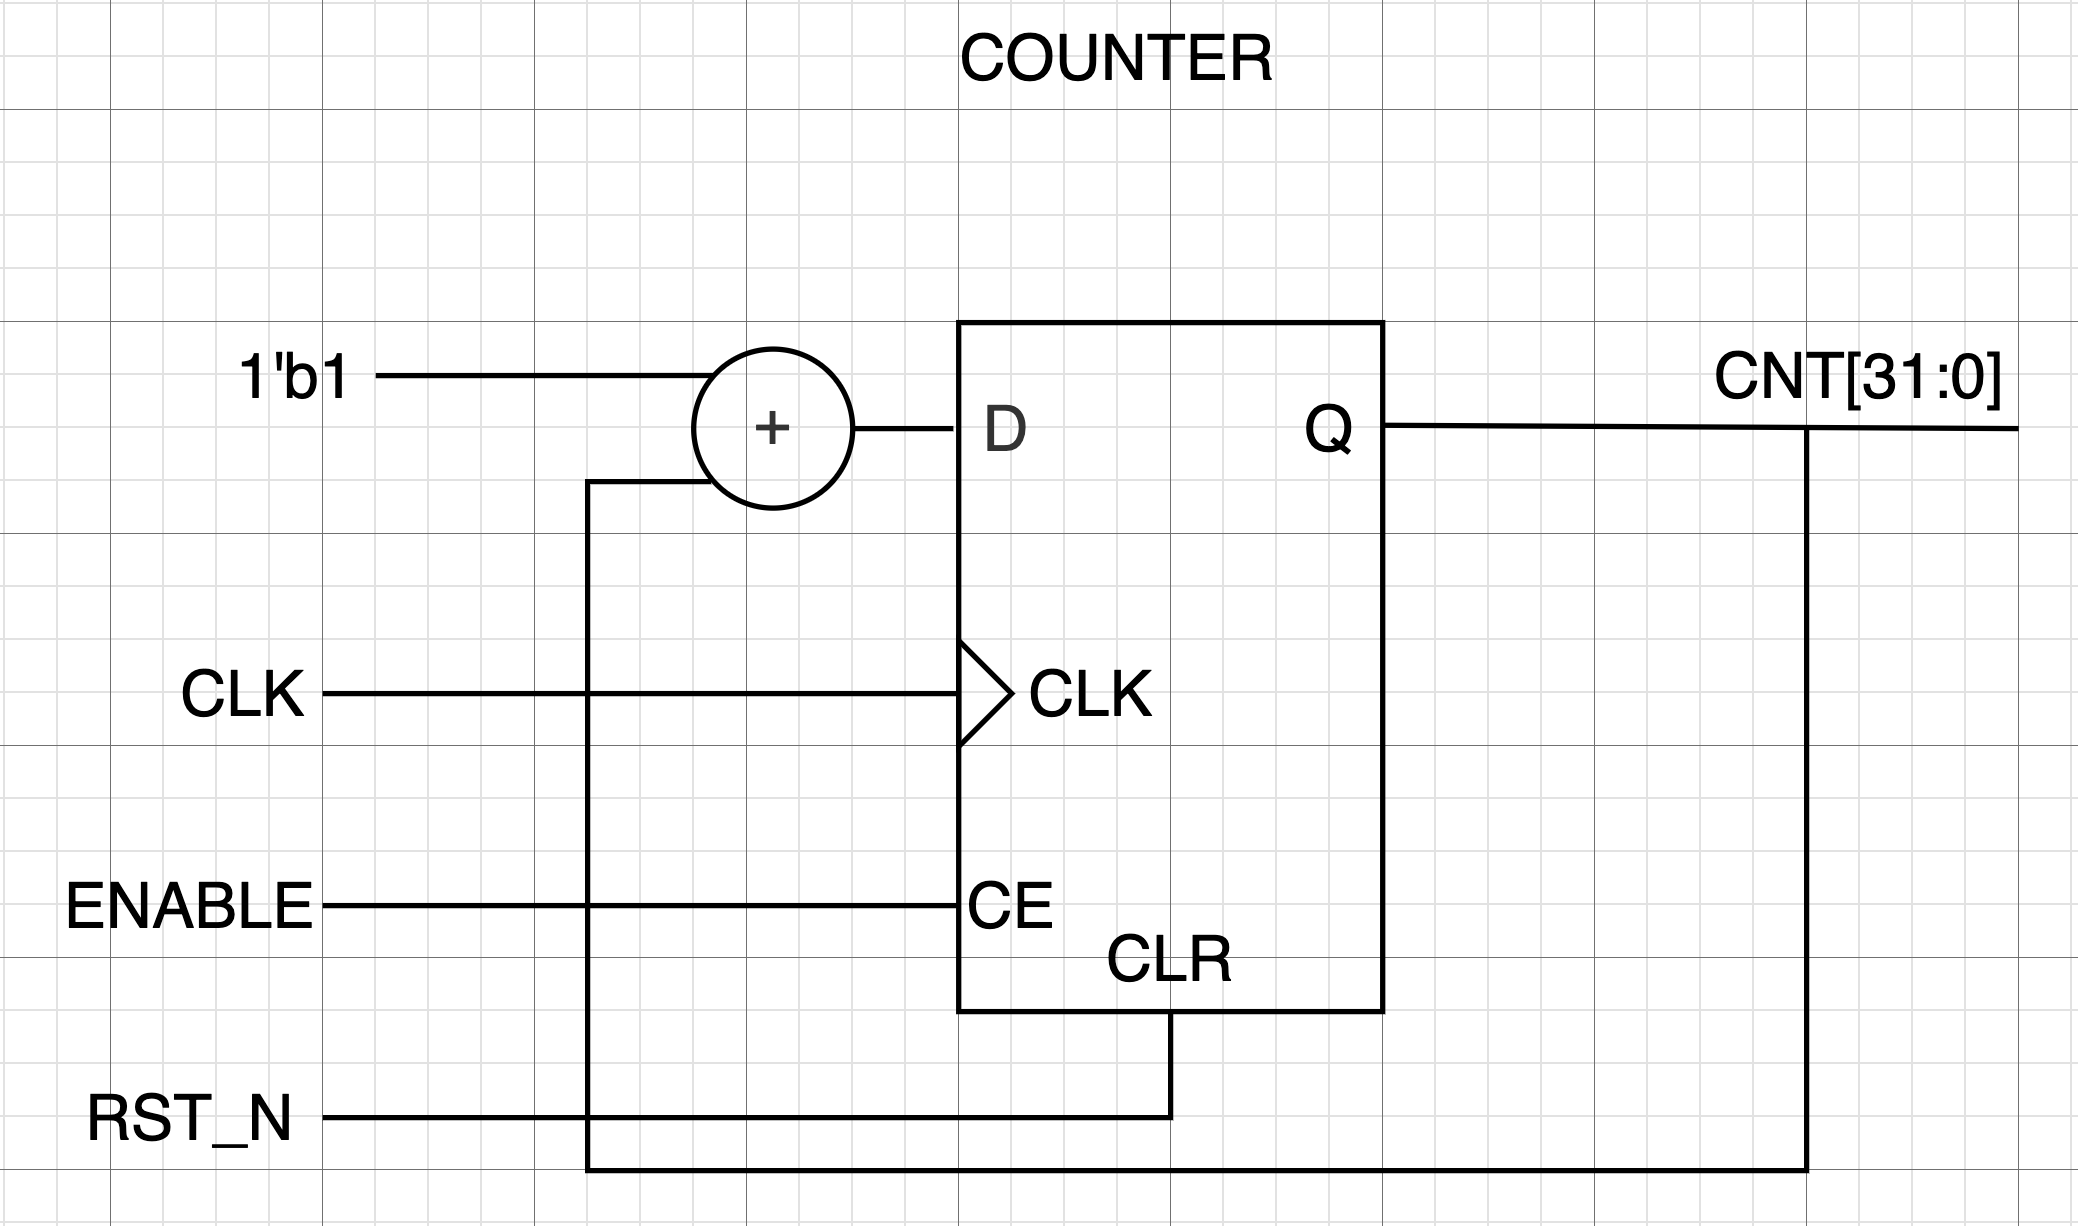
\includegraphics[width=\textwidth]{image/counter.png}
  \caption{Синхронный счетчик по переднему фронту с асинхронным сбросом и сигналом разрешения, 32 разряда.}
\end{figure}
\begin{figure}[H]
    \centering
    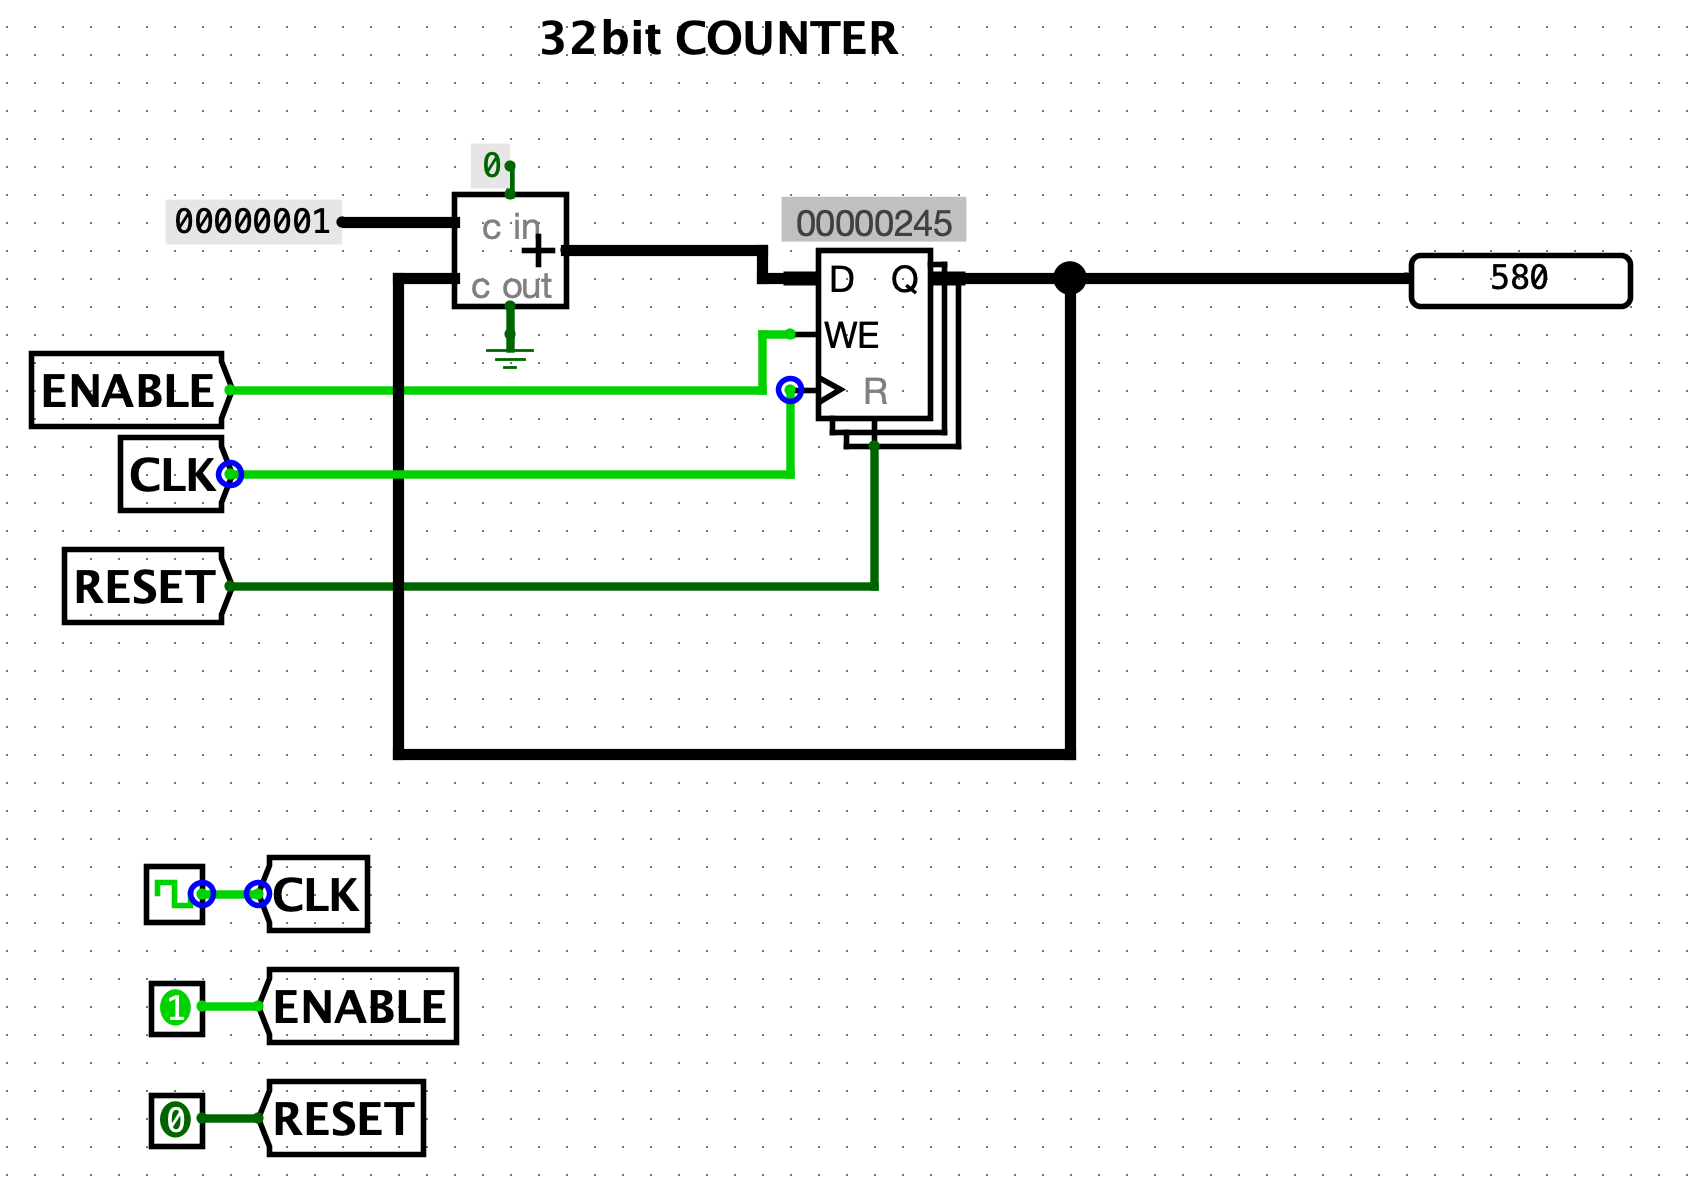
\includegraphics[width=\textwidth]{image/counter-d.png}
    \caption{Синхронный счетчик по переднему фронту с асинхронным сбросом и сигналом разрешения, 32 разряда.}
\end{figure}

Счетчик тактируется от CLK по переднему фронту. Когда уровень enable высокий,
то счетчик инкрементируется, когда уровень низкий — счетчик сохраняет свое
значение с предыдущего такта. 

По заднему фронту rst\_n счетчик асинхронно сбрасывается в 0.

На выходе счетчика по переднему фронту выставляется значение $Q(t-1) + 1$ по модулю разрядности счетчика.
\subsubsection{Разработанный модуль}
\lstinputlisting[style=verilog, language=verilog]{../src/counter/src/counter.v}
\subsubsection{Тестовый план:}
Области эквивалентности:
\begin{itemize}
  \item enable = 1, rst\_n = 1 -- инкремент
  \item enable = 1, rst\_n = 0 -- сброс
  \item enable = 0, rst\_n = 1 -- сохранение значения
\end{itemize}
\lstinputlisting[style=verilog, language=verilog]{../src/counter/src/counter_tb.v}
\textbf{Результаты тестирования:}

\begin{lstlisting}[language=verilog]
  [T=720] All tests passed
\end{lstlisting}

\begin{figure}[H]
  \centering
  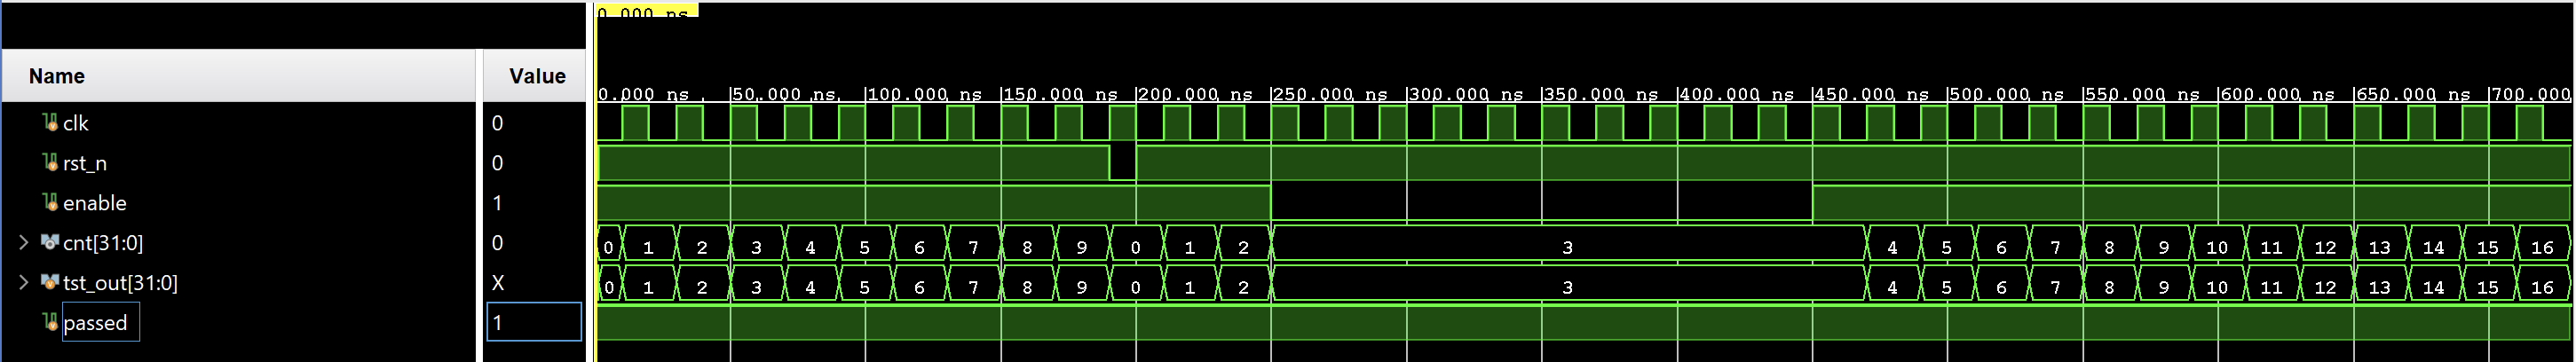
\includegraphics[width=\textwidth]{image/counter-diagram.png}
  \caption{Временная диаграмма работы счетчика}
\end{figure}

\subsection{Сдвиговый регистр}
\begin{figure}[H]
  \centering
  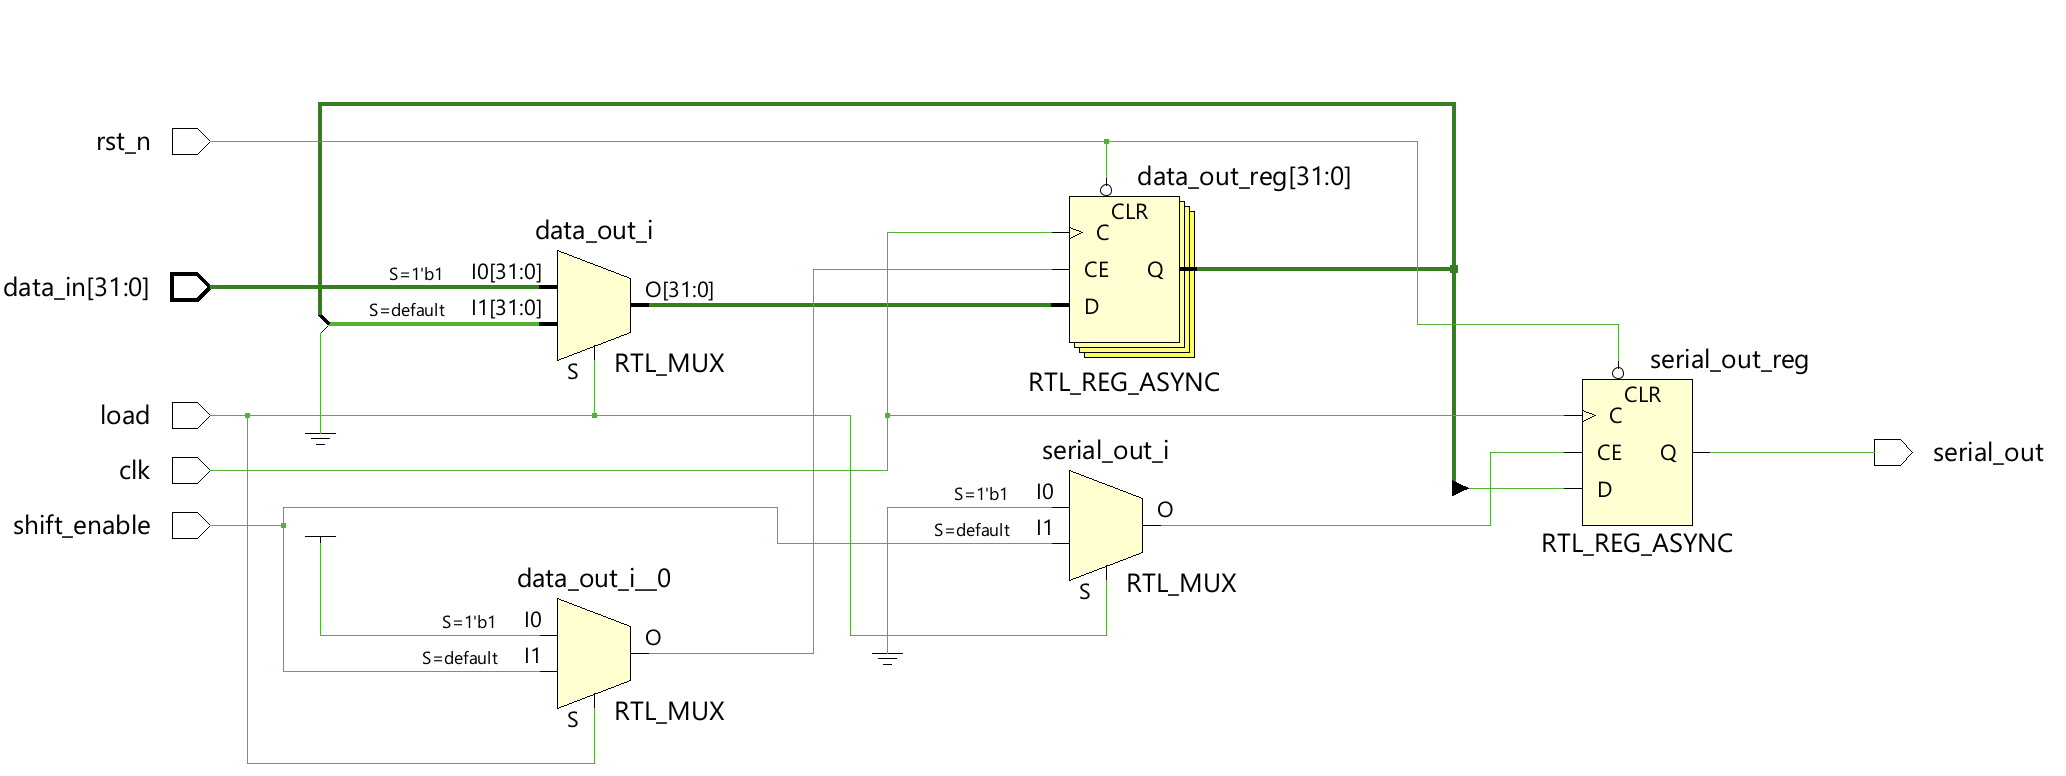
\includegraphics[width=\textwidth]{image/shift-right.png}
  \caption{Схема сдвигового регистра с параллельной загрузкой и последовательным сдвигом вправо}
\end{figure}
\begin{figure}[H]
    \centering
    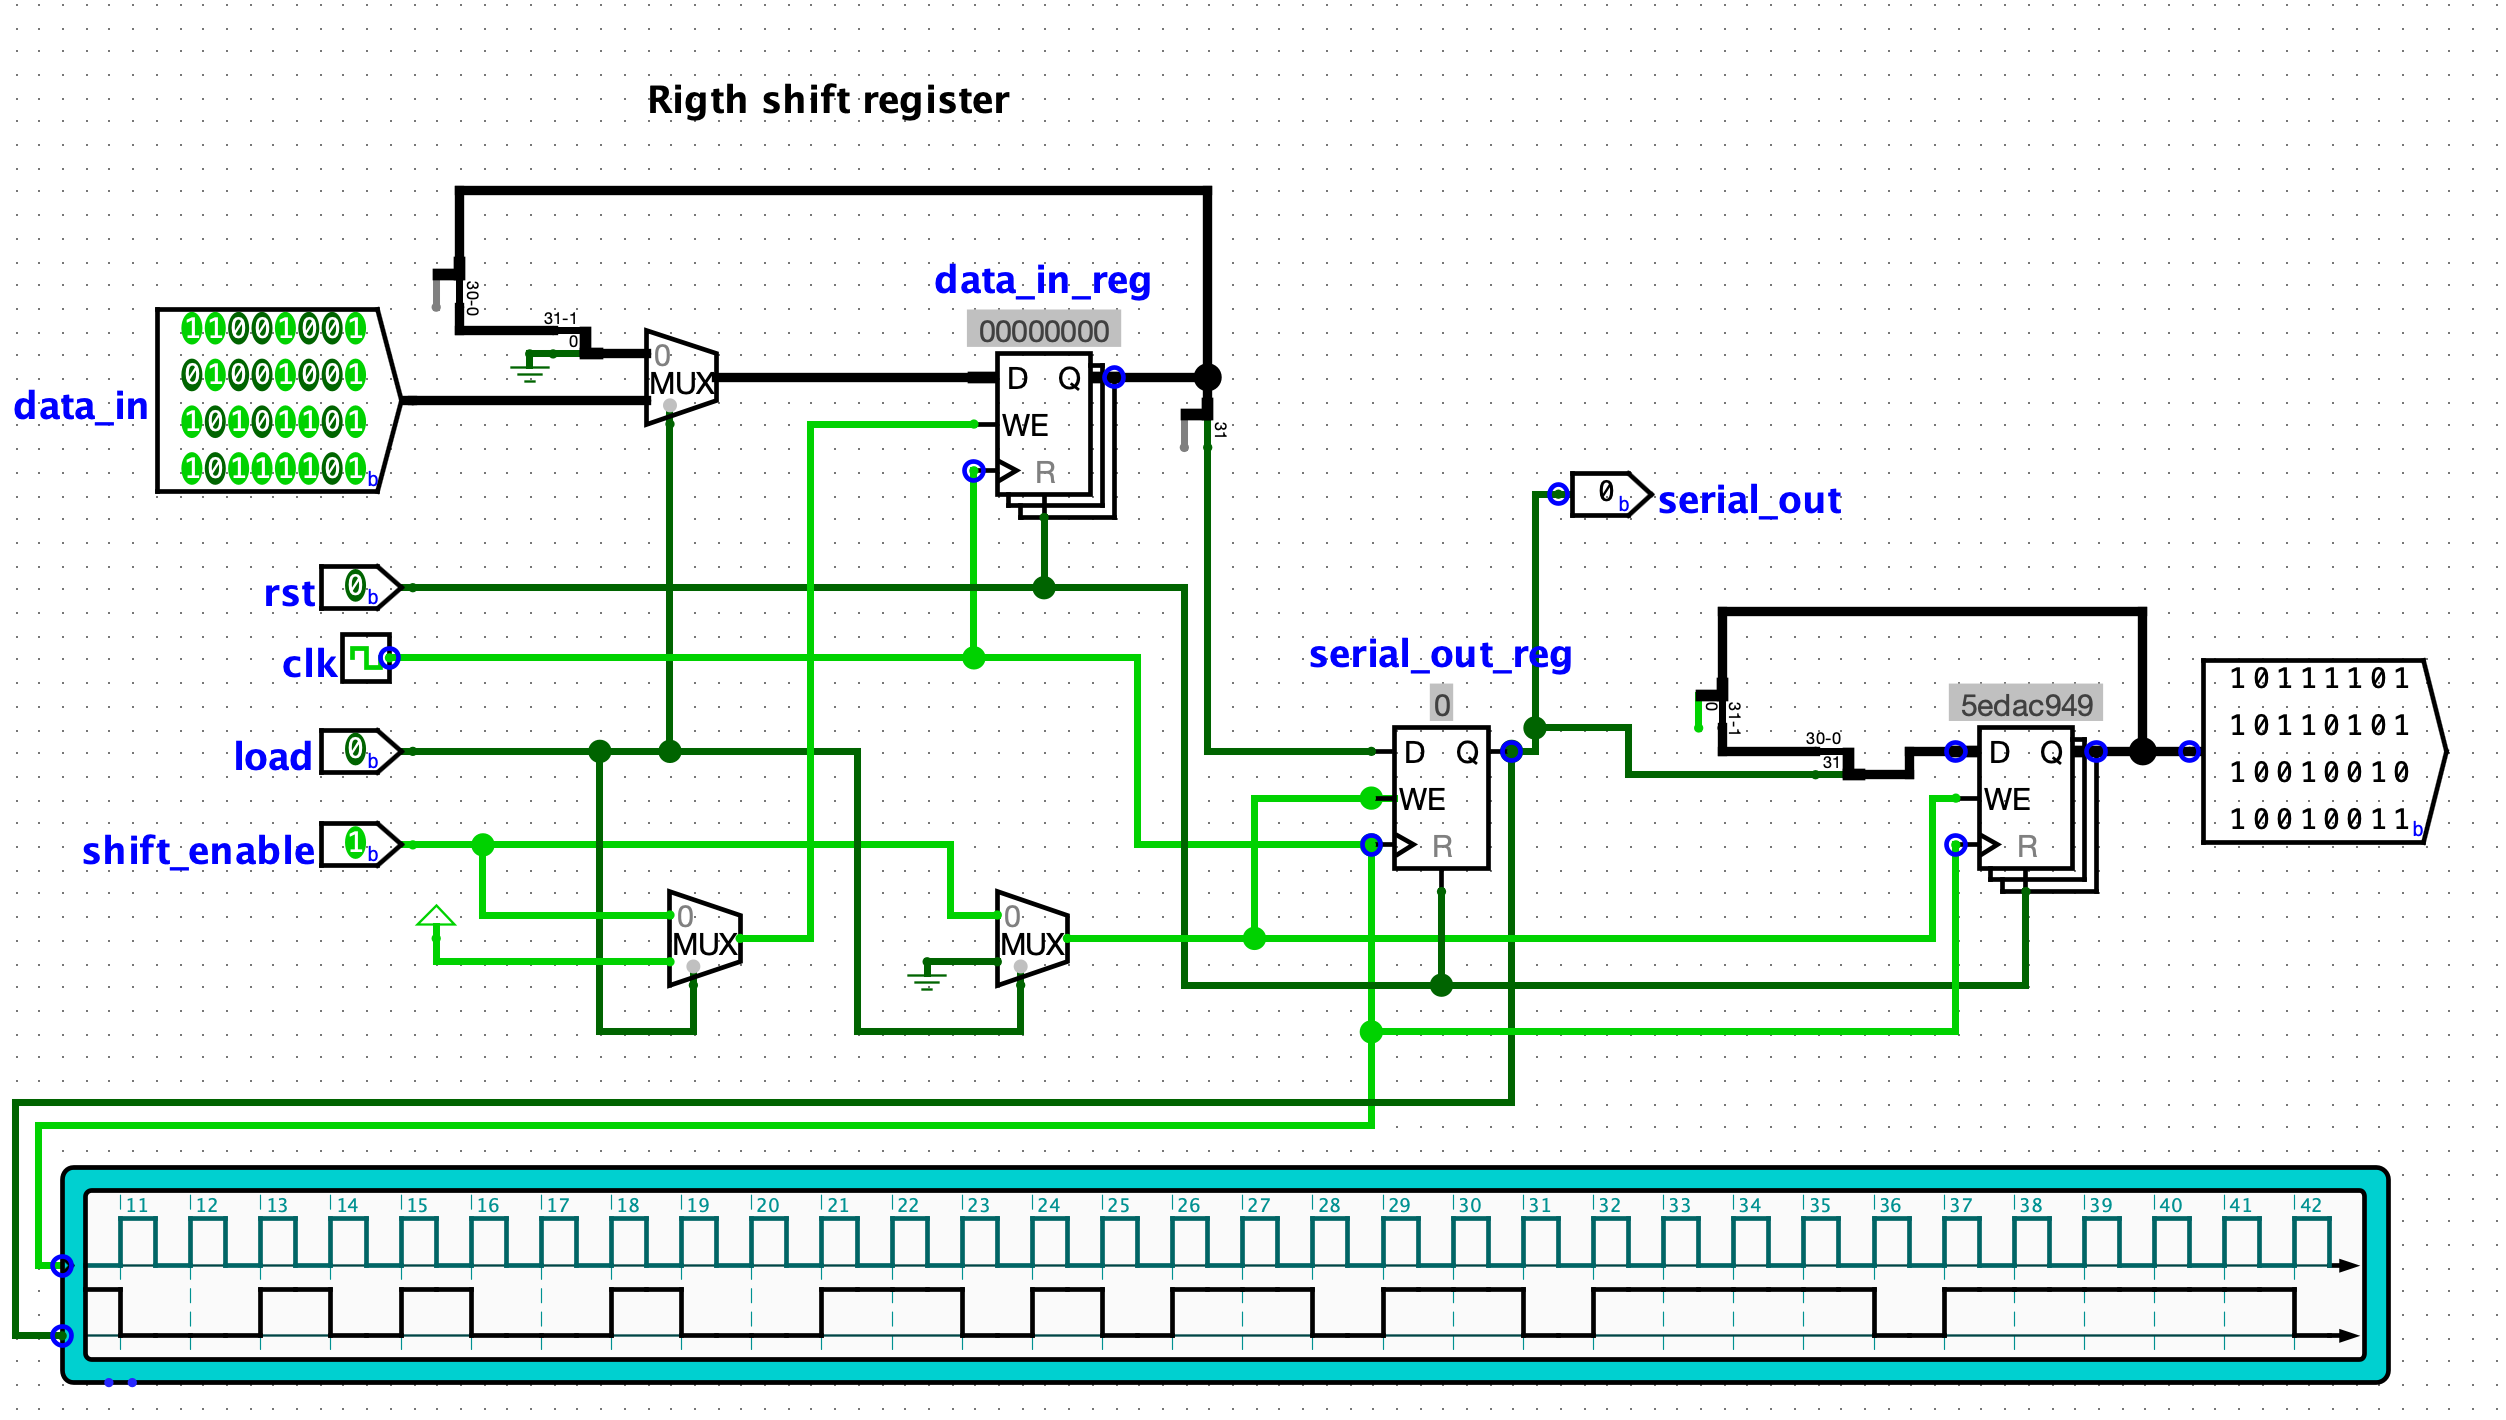
\includegraphics[width=\textwidth]{image/right-shift-reg.png}
    \caption{Схема сдвигового регистра с параллельной загрузкой и последовательным сдвигом вправо}
  \end{figure}
Сдвиговый регистр с параллельной загрузкой и последовательным сдвигом вправо.
Каждый фронт тактового сигнала, при наличии активного сигнала разрешения, выполняется операция сдвига вправо.
При наличии активного сигнала загрузки, в регистр загружается значение с входа D.
По заднему фронту сигнала сброса, регистр сбрасывается в 0.
\subsubsection{Разработанный модуль}
\lstinputlisting[style=verilog, language=verilog]{../src/shift_right/src/shift_right.v}
\subsubsection{Тестовый план:}
\begin{enumerate}
  \item Протестировать сдвиг при пустом буффере.
  \item Протестировать сброс регистра.
  \item Протестировать загрузку значения в регистр.
  \item Протестировать сдвиг данных после сброса.
\end{enumerate}
\begin{figure}[H]
  \centering
  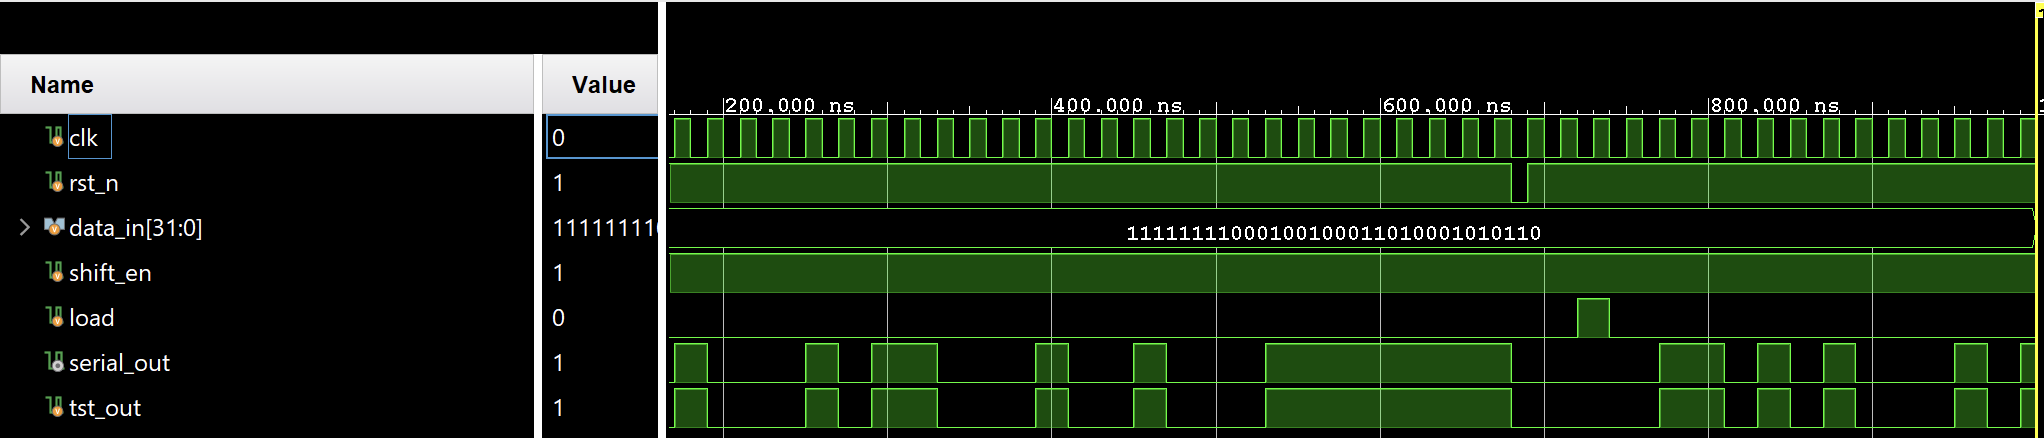
\includegraphics[width=\textwidth]{image/shift-right-diagram.png}
  \caption{Временная диаграмма работы сдвигового регистра}
\end{figure}
\lstinputlisting[style=verilog, language=verilog]{../src/shift_right/src/shift_right_tb.v}
\textbf{Результаты тестирования:}
\begin{lstlisting}[language=verilog]
#################### Starting simulation ####################
########## TEST: Load value ##########
########## TEST: Reset ##########
########## TEST: Buffer is empty ##########
########## TEST: Shift right continue ##########
[T=1060] All tests passed
\end{lstlisting}
 
\subsection{Конечный автомат}

Схема конечного автомата

\begin{figure}
    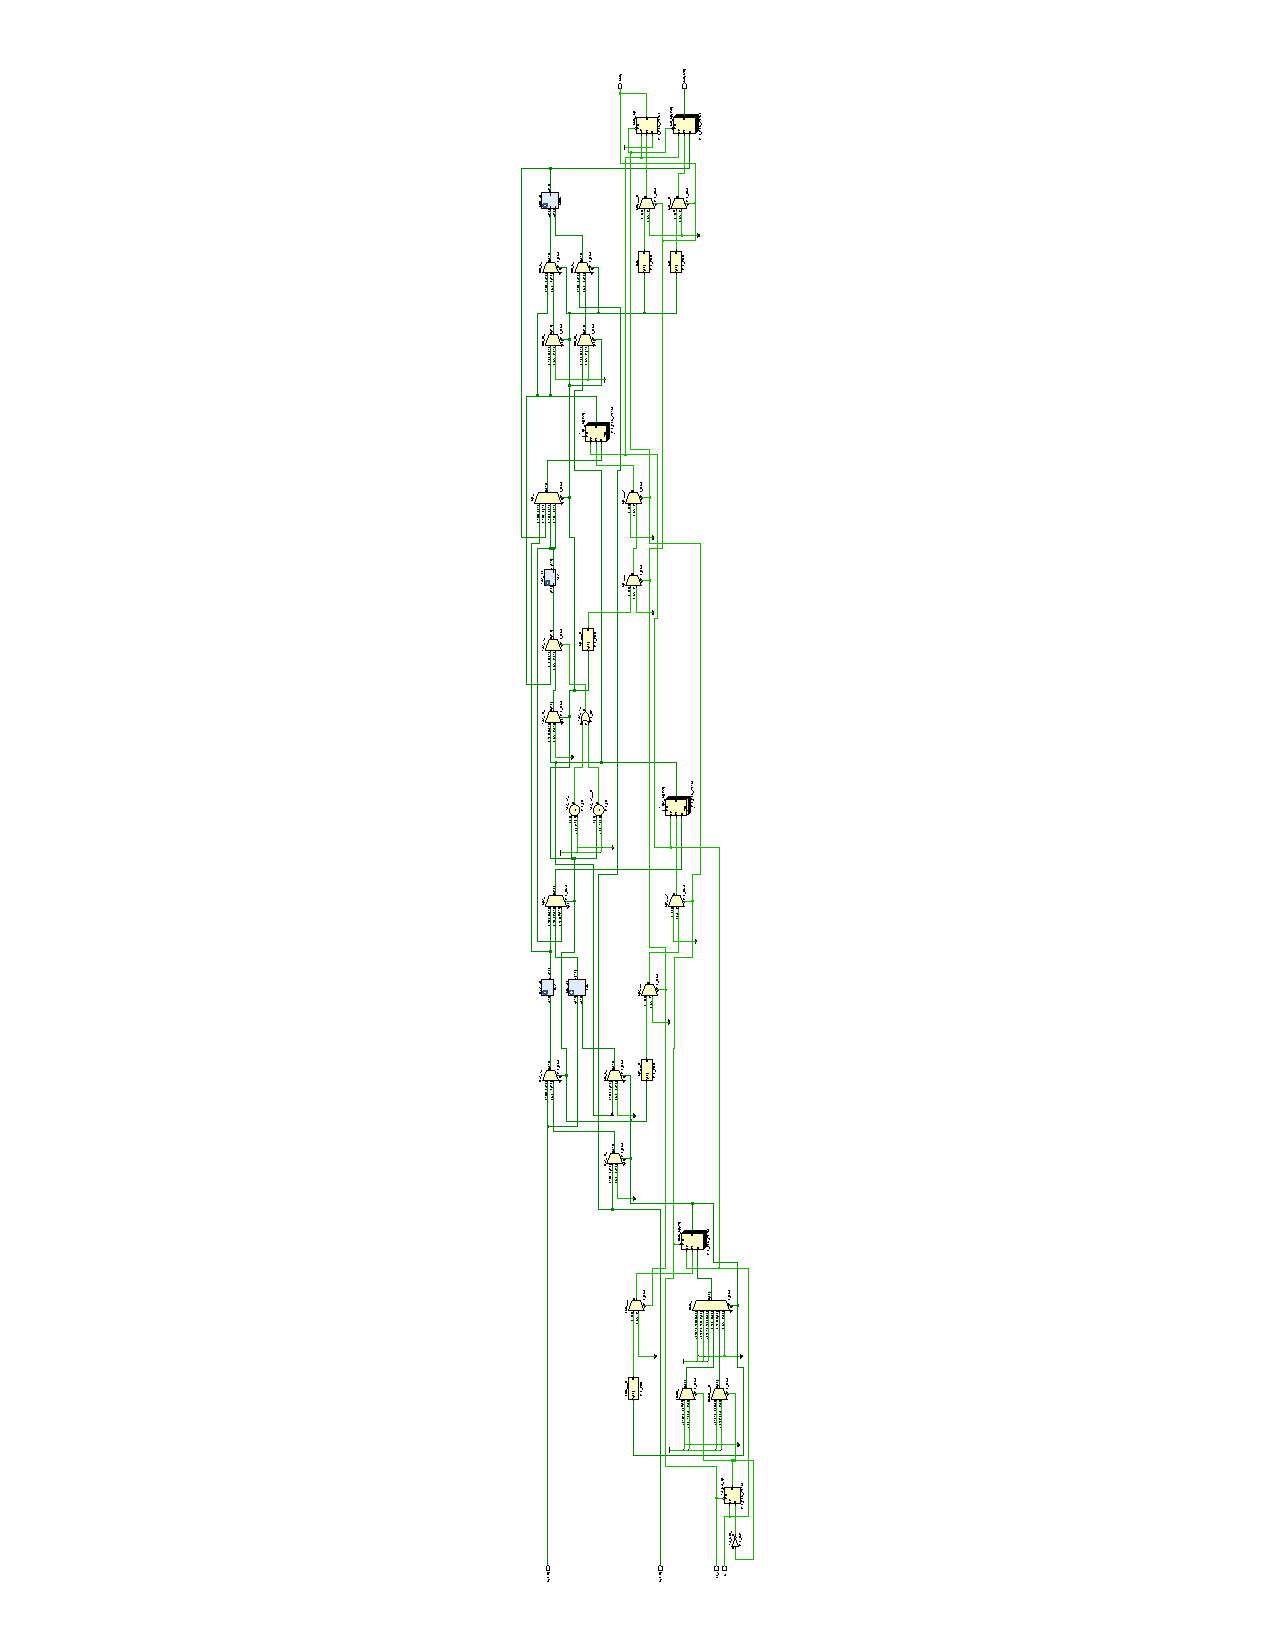
\includegraphics[]{image/fsm-schema.pdf}
\end{figure}

Конечный автомат состоит из 7 состояний, которые соответвуют последовательным этапам вычисления функции $(A/2+B)*8 + (A-B/2)*4$.
Чтобы автомат перешел в начальное состояние, необходимо подать сигнал сброса rst.
Когда автомат закончит работу он устанавливает сигнал ready в 1 и переходит в первое состояние, где ожидает сигнала сброса.
\subsubsection{Разработанный модуль}
\textbf{Сумматор}
\lstinputlisting[style=verilog, language=verilog]{../src/fsm/src/adder.v}
\textbf{Делитель на 2}
\lstinputlisting[style=verilog, language=verilog]{../src/fsm/src/div2.v}
\textbf{Умножитель на 8}
\lstinputlisting[style=verilog, language=verilog]{../src/fsm/src/mul2.v}
\textbf{Вычитатель}
\lstinputlisting[style=verilog, language=verilog]{../src/fsm/src/sub.v}
\textbf{Конечный автомат}
\lstinputlisting[style=verilog, language=verilog]{../src/fsm/src/fsm.v}
\subsubsection{Тестовый план:}
\begin{enumerate}
  \item Протестировать правильность вычисления функции на любых валидных входных данных.
  \item Протестировать сброс автомата.
  \item Протестировать максимальные значения входных аргументов. $a = 2^{32} - 1~ and~ b = 2^{32} - 1$
  \item Протестировать значения 0 входных аргументов. $a = 0 and b = 0$
  \item Протестировать минимальные значения входных аргументов. $a = -2^{31}~ and~ b = -2^{31}$
\end{enumerate}
\lstinputlisting[style=verilog, language=verilog]{../src/fsm/src/fsm_tb.v}
\textbf{Результаты тестирования:}
\begin{lstlisting}[language=verilog]
[T=0] Test 1: a = 6, b = 4
[T=250] Test 2: Reset
[T=530] Test 3: a = 2^32 - 1, b = 2^32 - 1
[T=550] Test 4: a = 0, b = 0
[T=830] Test 5: a = -2^31, b = -2^31
[T=1110] All tests passed
\end{lstlisting}


\begin{figure}[H]
  \centering
  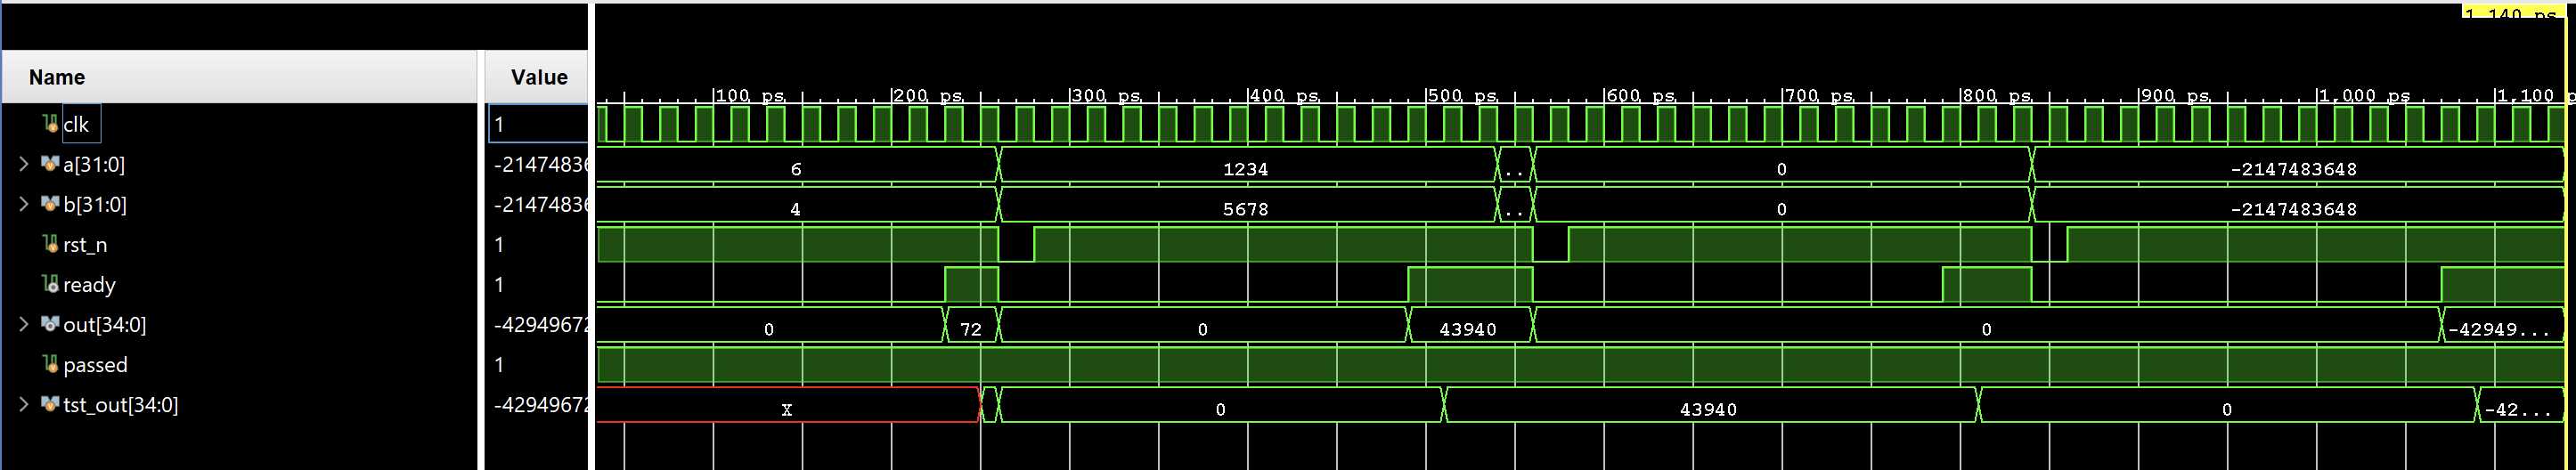
\includegraphics[width=\textwidth]{image/fsm-diagram.png}
  \caption{Временная диаграмма работы конечного автомата}
\end{figure}

\subsection{Делитель частоты}
\begin{figure}[H]
  \centering
  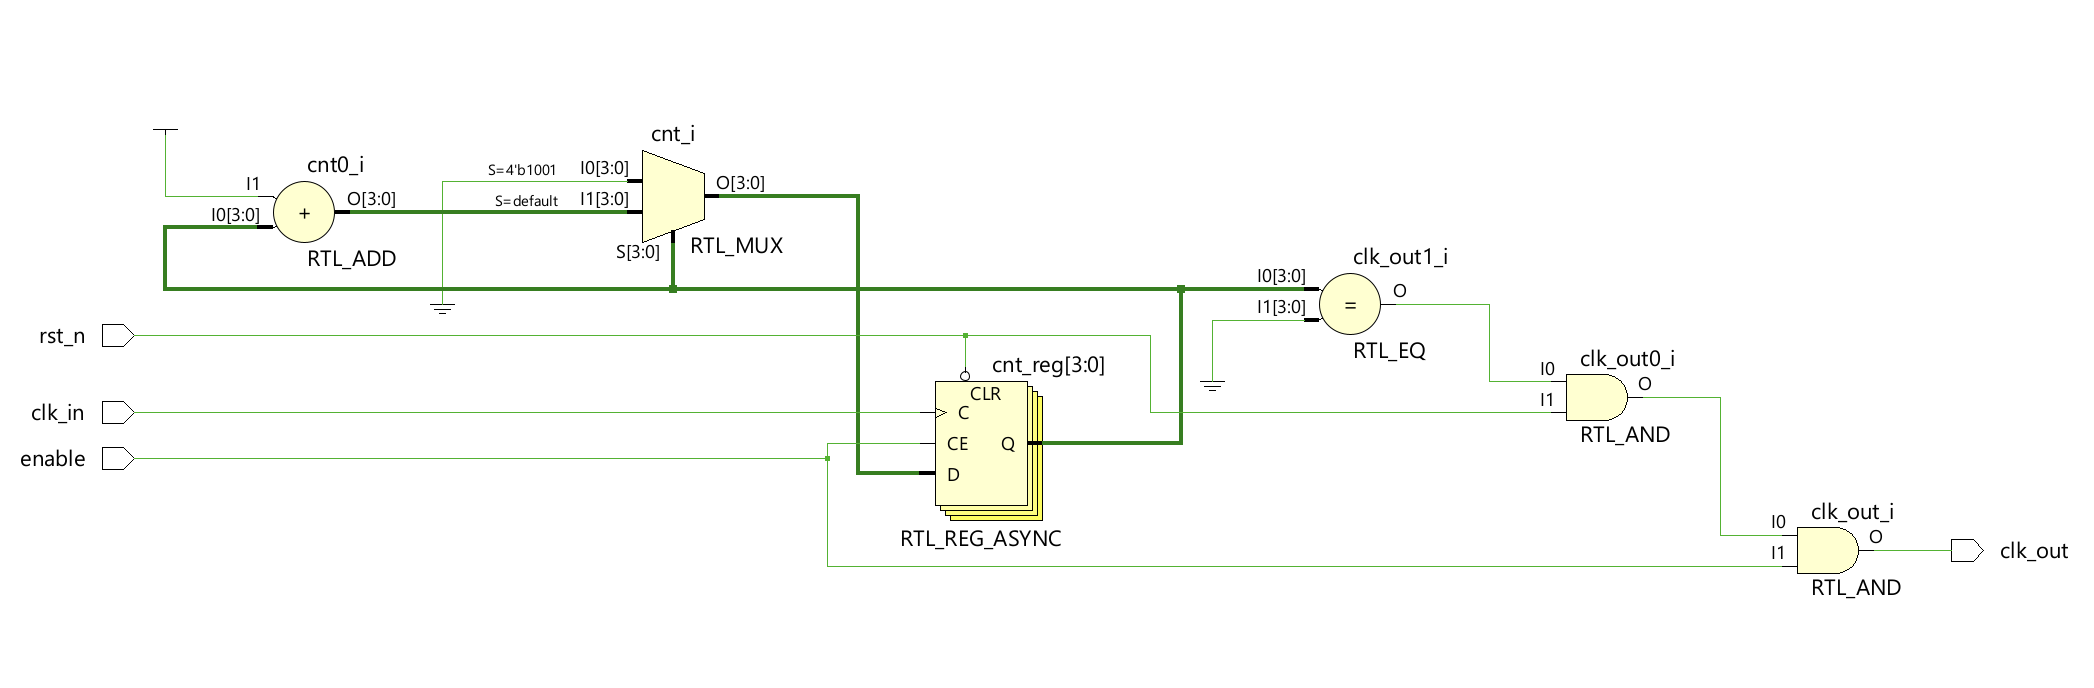
\includegraphics[width=\textwidth]{image/freq-div.png}
  \caption{Схема делителя частоты, уменьшает частоту на 10 раз}
\end{figure}
\begin{figure}[H]
    \centering
    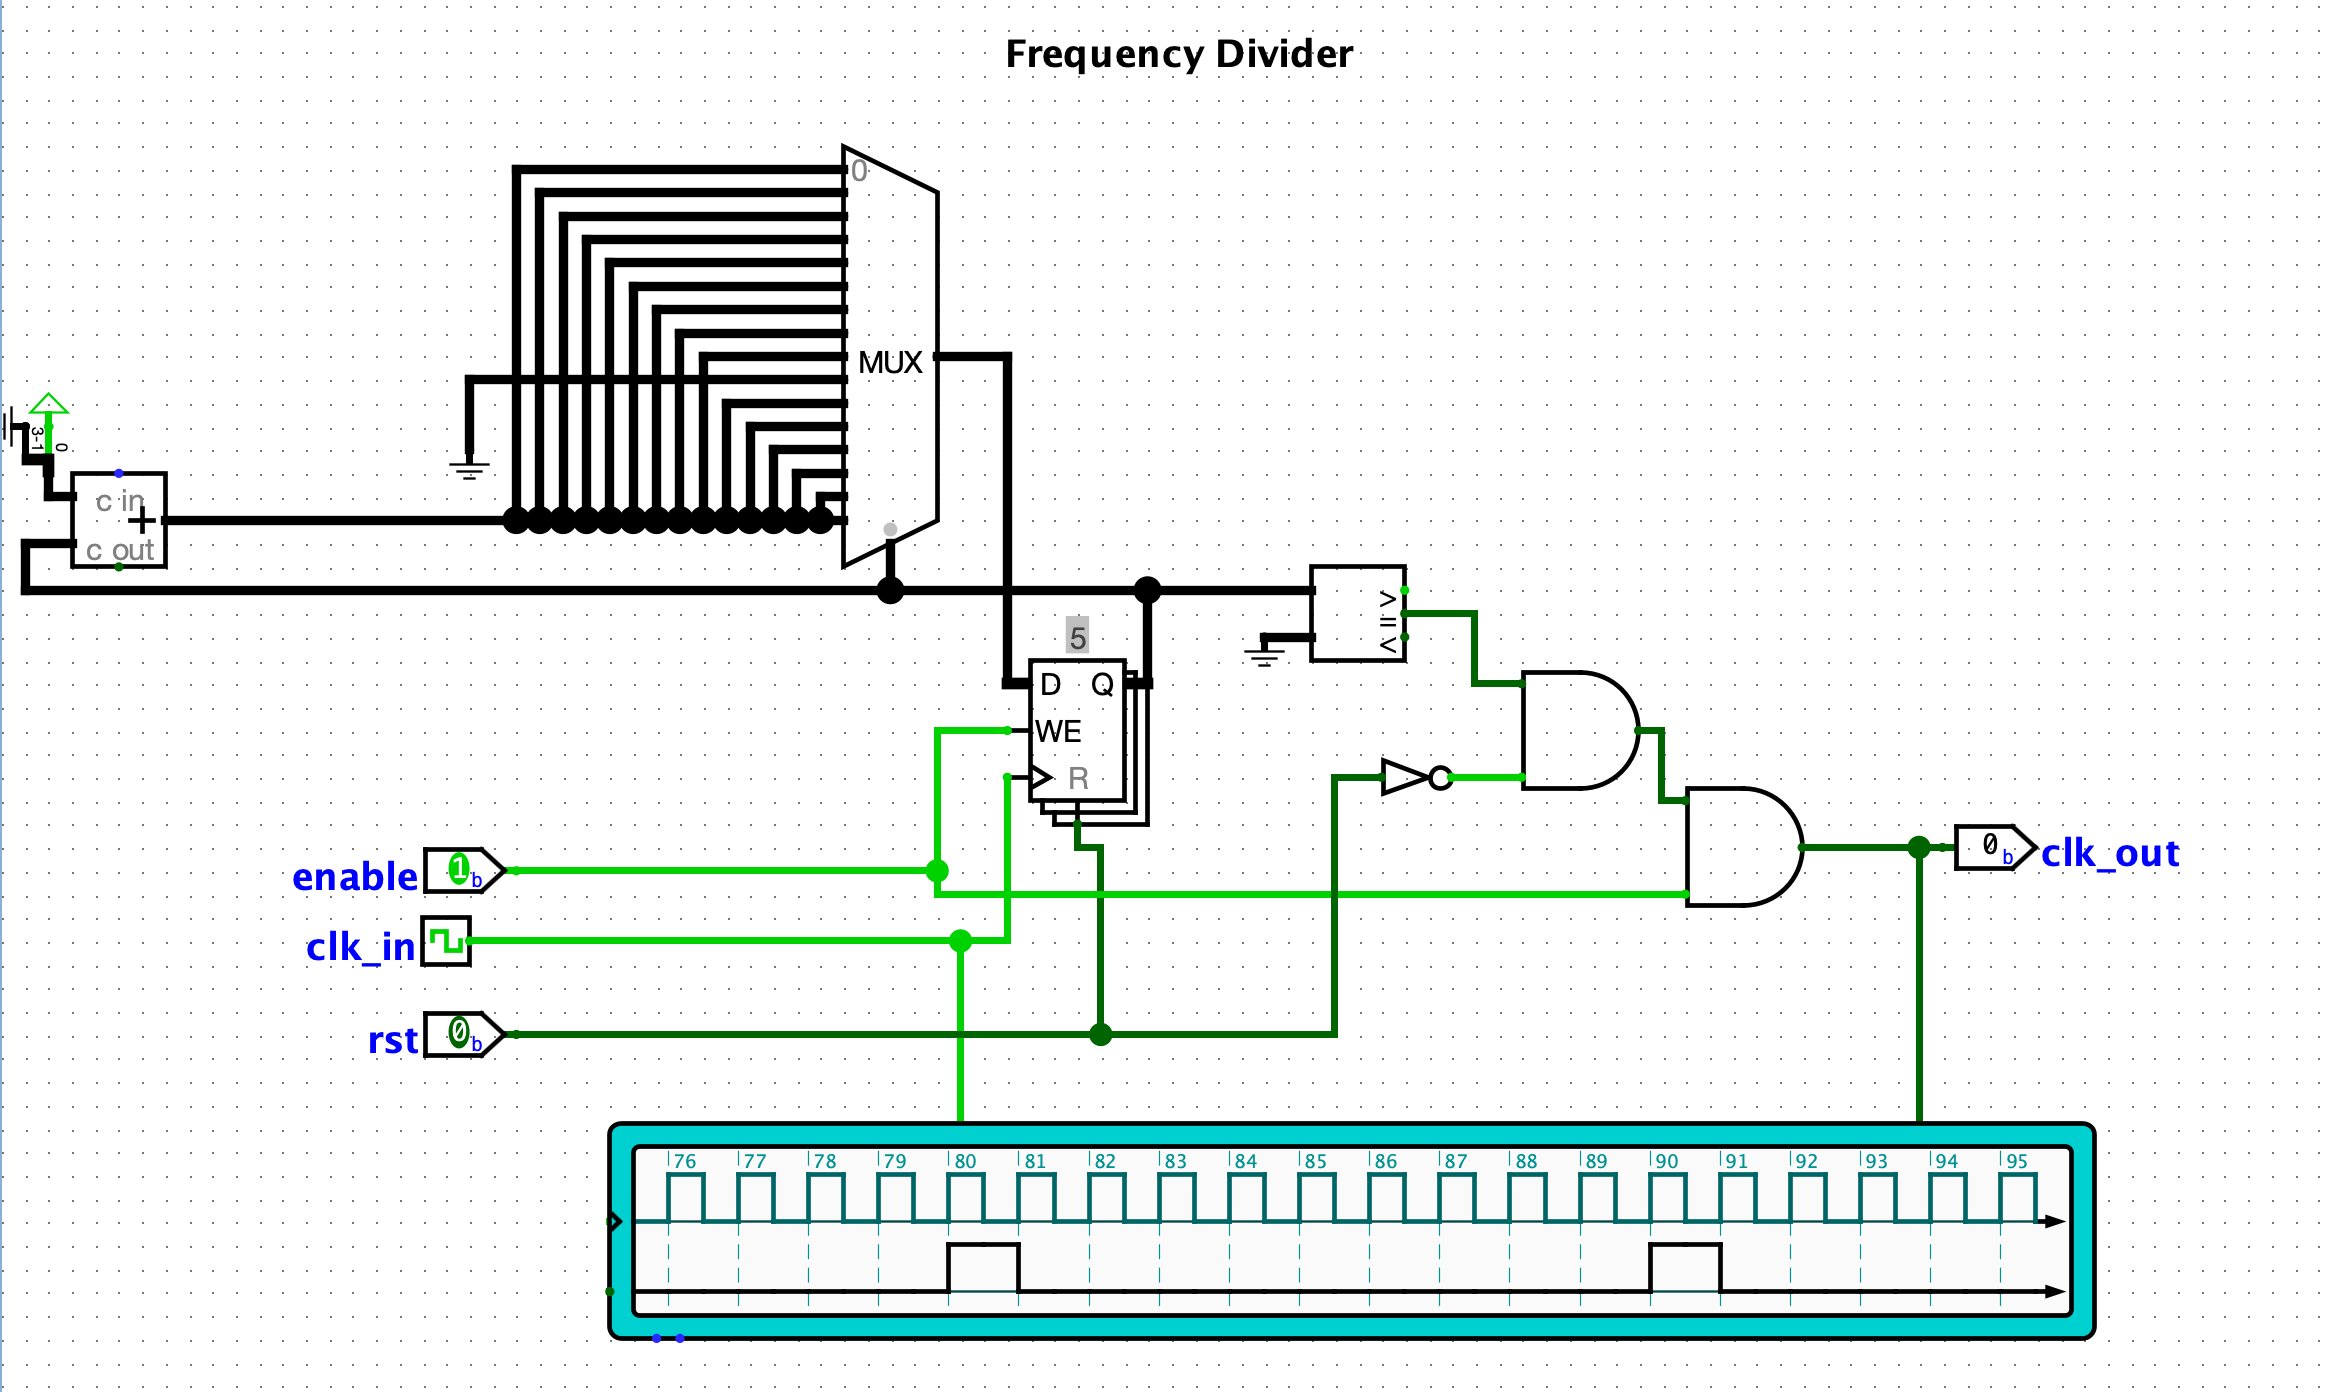
\includegraphics[width=\textwidth]{image/frequency-div.png}
    \caption{Схема делителя частоты, уменьшает частоту на 10 раз}
  \end{figure}

При подаче асинхронного сигнала сброса rst d-триггер сбрасывается.
С каждым тактом инкрементируется значение регистра cnt\_reg до тех пор, пока cnt не станет равным значению DIV\_CNT-1. 
Тогда значение регистра clk\_out становиться равным 1 и обнуляется значение cnt.
\subsubsection{Разработанный модуль}
\lstinputlisting[style=verilog, language=verilog]{../src/freq_div/src/freq_div.v}
\subsubsection{Тестовый план:}
\begin{enumerate}
  \item Протестировать правильное деление частоты на 10.
  \item Протестировать сброс делителя.
  \item Протестировать сигнал разрешения.
  \item Протестировать продолжение работы после сброса.
\end{enumerate}
\lstinputlisting[style=verilog, language=verilog]{../src/freq_div/src/freq_div_tb.v}
\begin{figure}[H]
  \centering
  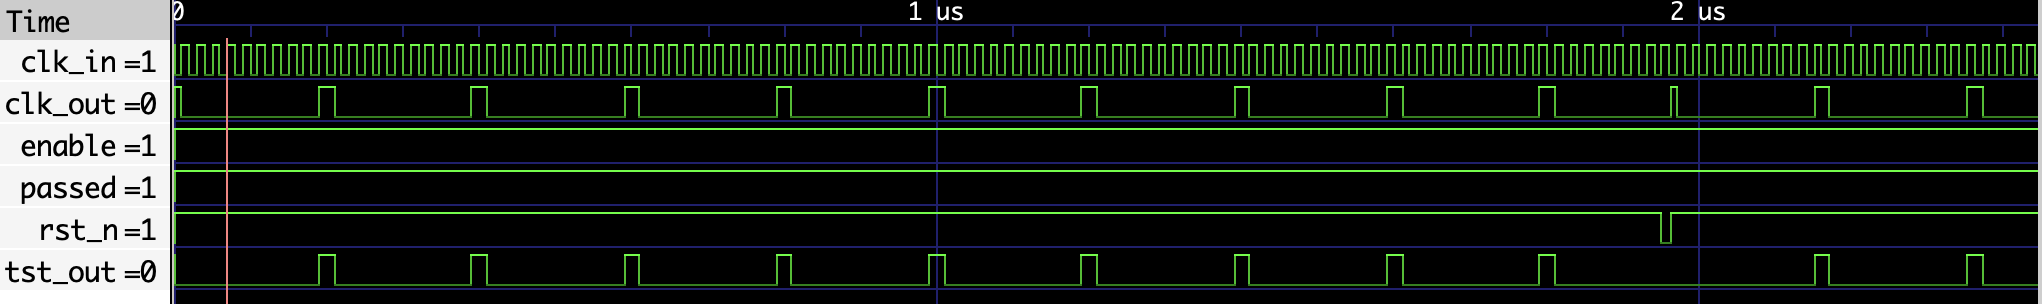
\includegraphics[width=\textwidth]{image/freq-div-diagram.png}
  \caption{Временная диаграмма работы делителя частоты}
\end{figure}

\textbf{Результаты тестирования:}

\begin{lstlisting}[language=verilog]
[T=1] Test 1: Count test
[T=1940] Test 2: Reset, Should Be 0
[T=1961] Test 3: Continue count
[T=3900] Test 4: Enable disable
[T=5760] All tests passed
\end{lstlisting}

\section{Функция COUNT FREE}
\begin{figure}[H]
  \centering
  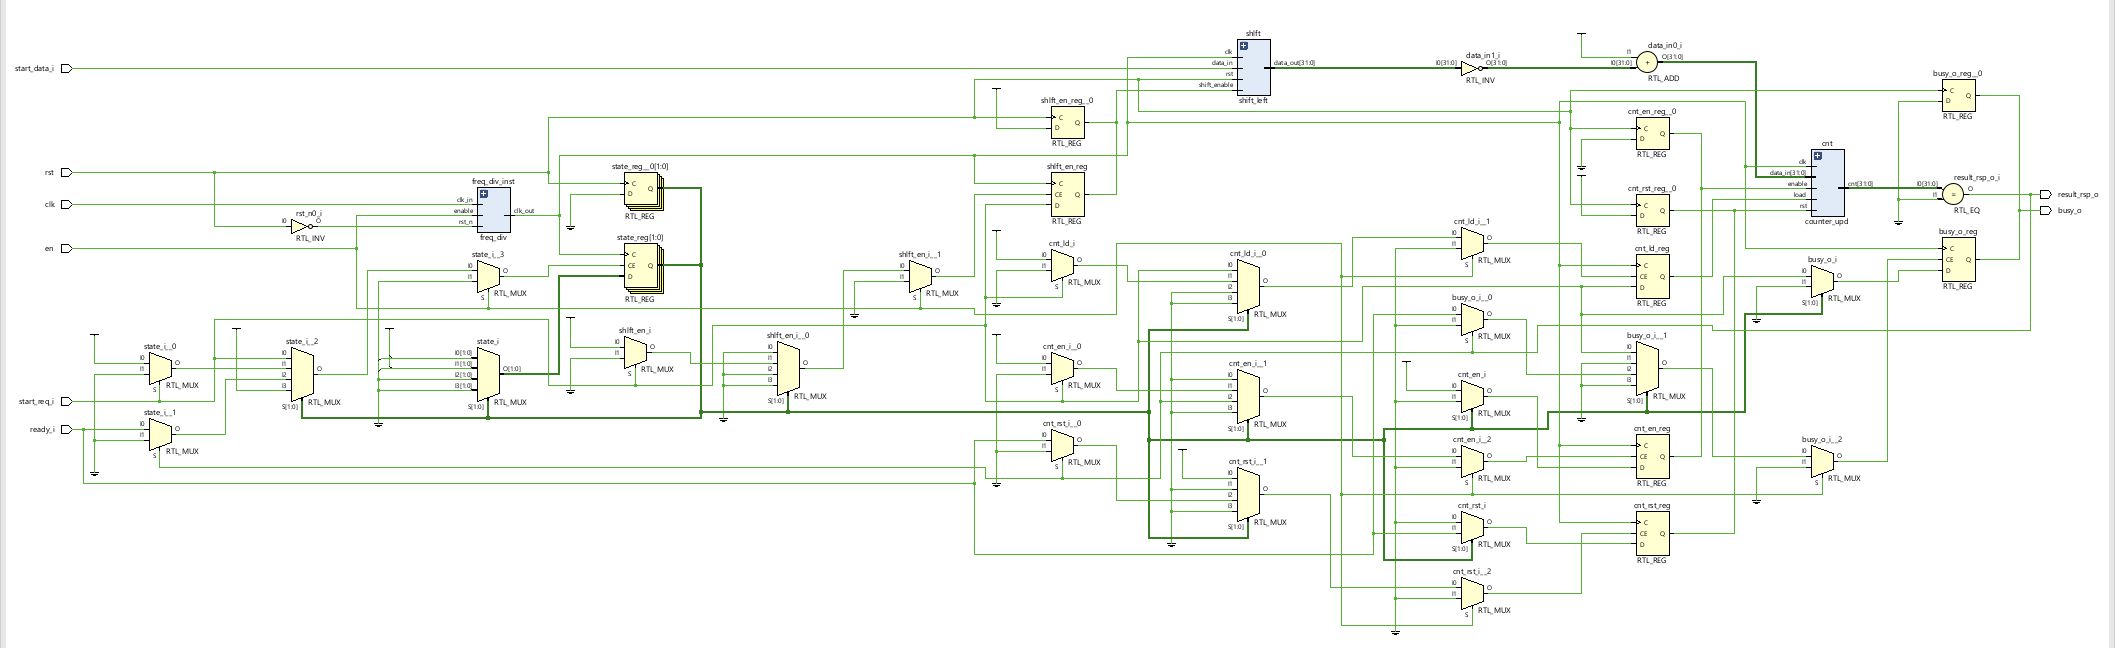
\includegraphics[width=\textwidth]{image/count-free.png}
  \caption{Схема функции COUNT\_FREE}
\end{figure}
\textbf{Результаты тестирования:}
\begin{lstlisting}[language=verilog]
  [T=0] Test 1: Reset
  [T=222] Test 2: Count
  [T=4440] All tests passed
\end{lstlisting}


\section{FIFO}
\begin{figure}[H]
  \centering
  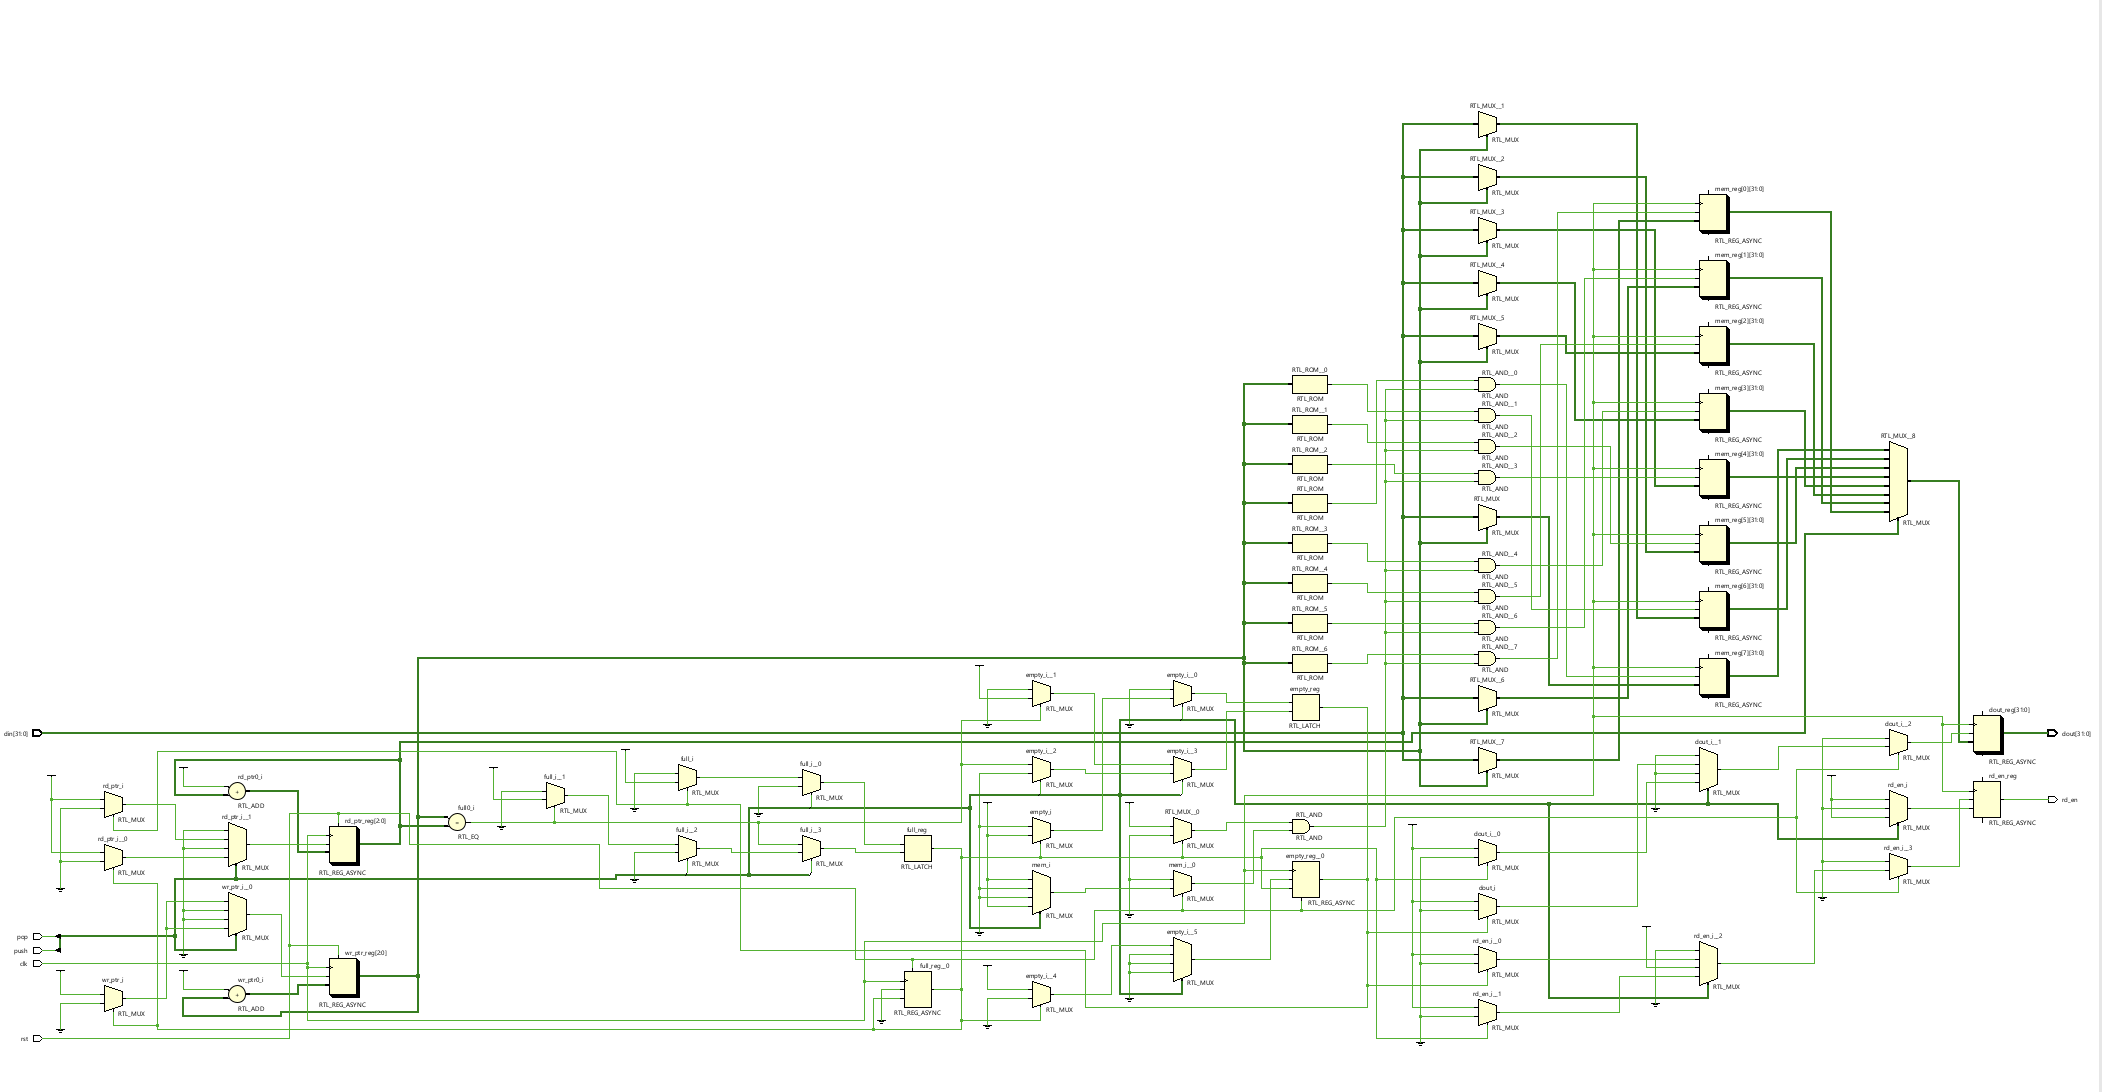
\includegraphics[width=\textwidth]{image/fifo.png}
  \caption{Схема FIFO}
\end{figure}
\textbf{Результаты тестирования:}
\begin{lstlisting}[language=verilog]
Test 1: Basic write/read
Test 2: Overflow condition
Test 3: Underflow condition
Test 4: PUSH and POP on the same clock cycle
[T=675] All tests passed
\end{lstlisting}


\section{Вывод}
В ходе выполнения лабораторной работы были разработаны и протестированы следующие устройства:
\begin{itemize}
  \item Счетчик с асинхронным сбросом и сигналом разрешения.
  \item Сдвиговый регистр с параллельной загрузкой и последовательным сдвигом вправо.
  \item Конечный автомат, вычисляющий функцию $(A/2+B)*8 + (A-B/2)*4$.
  \item Делитель частоты, уменьшающий частоту на 10 раз.
  \item Устройство COUNT\_FREE, считающее количество единиц во входном потоке.
  \item FIFO, реализующая очередь с фиксированным размером.
\end{itemize}
Вопрос: На что влияет не учитывание всех учитывать всех
возможных комбинации входных данных?

Ответ:

    В комбинационной логике это ни на что не влияет. 








\end{document}